\documentclass[12pt,fleqn]{article}\usepackage{../common}
\begin{document}
Ders 7

Bugunun konusu ``hersey''. Simdiye kadar gordugumuz her sey
yani. Vektorleri gorduk, noktasal carpimlari (dot product) gorduk. Iki
vektorun noktasal carpimi

\[ \vec{A} \cdot \vec{B} = \sum a_ib_i\]

yani o vektorlerin tum elemanlarinin sirasiyla birbiriyle carpilip
toplanmasi. O da suna esit

\[ |\vec{A}||\vec{B}| \cos \theta \]

Noktasal carpimi acilari olcmek icin kullanabiliriz, eger $\cos \theta$
terimini tek basina birakirsak, geri kalanlari cozeriz. Bu sekilde iki
vektorun dik olup olmadigini da anlariz. Cunku o zaman sonuc sifir olur, ve
$\cos \theta = 0$ ise aci dik demektir. 

Gordugumuz bir diger kavram capraz carpim (cross product) kavramiydi. 

\[ \vec{A} \times \vec{B} = 
\left|\begin{array}{rrr}
\vec{i} & \vec{j} & \vec{k}  \\
a_1 & a_2 & a_3 \\
b_1 & b_2 & b_3 
\end{array}\right|
\]

Esitligin sagindaki determinant isareti, matris isareti degil, buna
dikkat. Capraz carpimin uygulamalari uzayda bir ucgenin alanin bulmak
mesela. 

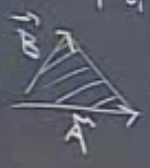
\includegraphics[height=2cm]{7_1.png}

Bu alan

\[ \frac{1}{2}|\vec{A} \times \vec{B}| \]

ile hesaplanir. Cunku $|\vec{A} \times \vec{B}|$ bir paralelogram verir, onun yarisi 
aradigimiz ucgenin alanidir.

Capraz carpimin bir diger uygulama alani iki vektore ayni anda dik olan
ucuncu bir vektoru bulmaktir. Ona baglantili olarak bir duzleme (plane) dik
olan bir vektoru bulmak, yani ``normal vektoru'' bulmak. Duzlemin formulu
nedir? 

\[ ax + by + cz  = d \]

Normal vektor ise $\vec{N} = <a,b,c>$ olarak gosterilir. Normal vektorun
degerleri duzlem formulune katsayi olarak giderler. 

Cizgiler

Cizgilerin formulu icin bir baslangic noktasina ve o cizgiye paralel olan
bir vektore ihtiyacimiz var. 

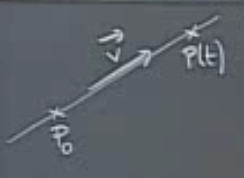
\includegraphics[height=2cm]{7_2.png}

\[ P(t) = P_0 + t \vec{v} \]

Problem 3

\[ A = 
\left[\begin{array}{rrr}
1 & 3 & 2 \\
2 & 0 & -1 \\
1 & 1 & 0
\end{array}\right]
 \]

Bize matrisin tersi verilmis ve iki oge bos birakilmis

\[ A^{-1} = \frac{1}{2}
\left[\begin{array}{rrr}
1 & .. & .. \\
-1 & -2 & 5 \\
2 & 2 & -6
\end{array}\right]
 \]

Yani bizden beklenen tersine cevirme islemini yapmak, ama bos birakilan
degerlere bakalim, bu noktada kafayi calistirip, sadece o noktalara tekabul 
eden minorleri hesaplamamiz bekleniyor. O minorler hangileri? Sunlar (x ile
isaretli). 

\[ A = 
\left[\begin{array}{rrr}
.. & .. & ..\\
x & .. & ..\\
x & .. & ..
\end{array}\right]
 \]

cunku devrigine alma islemini yapinca, o elemanlar A tersindeki nokta nokta olan
yere gecmis olacaklar. 

Minorleri hesaplarsak

\[ A = 
\left[\begin{array}{rrr}
.. & .. & ..\\
-2 & .. & ..\\
-3 & .. & ..
\end{array}\right]
 \]

Simdi kofaktorleri hatirlayalim (Ders 3)


\[ 
\begin{array}{rr}
+ - + \\
- + - \\
+ - + 
\end{array}
 \]

O zaman

\[ A = 
\left[\begin{array}{rrr}
.. & .. & ..\\
+2 & .. & ..\\
-3 & .. & ..
\end{array}\right]
 \]

Devrigini alalim

\[ A = 
\left[\begin{array}{rrr}
.. & +2 & -3\\
.. & .. & ..\\
.. & .. & ..
\end{array}\right]
 \]

Determinant'a bolelim. Determinantin ne oldugu verilmis, 2, ama bu deger zaten $1/2$
olarak $A$'nin tersi onunde duruyor. O zaman 2 ve -3 degerlerini oldugu gibi bos
olan yerlere tasiriz. 

\[ A^{-1} = \frac{1}{2}
\left[\begin{array}{rrr}
1 & 2 & -3 \\
-1 & -2 & 5 \\
2 & 2 & -6
\end{array}\right]
 \]


Ornek

$MX = 0$

Sistem

\[ x + 3y + z = 0 \]

\[ 2x - z  = 0\]

\[ x + y = 0 \]

Eger noktasal carpim olarak yazarsak 

\[ <x,y,z> \cdot <1,3,1> = 0 \]

\[ <x,y,z> \cdot <2,0,-1> = 0 \]

\[ <x,y,z> \cdot <1,1,0> = 0 \]

Bu ifade bize aslinda ustte sagdaki uc vektore dik olan bir vektoru bulmamizi
soyluyor, cunku o vektorle $<x,y,z>$ noktasal carpimi sifir sonucu veriyor. Iki
vektore dik ucuncu bir vektor bulmayi zaten biliyoruz, ilk iki vektor $<1,3,1>$
ve $<2,0,-1>$'i kullanarak bunu yapabiliriz, onlarin capraz carpimini aliriz
(ucuncu denklemi atliyoruz -aslinda hangi iki vektoru sectigimiz onemli degil-),

\[ 
\left|\begin{array}{rrr}
\vec{i} & \vec{j} & \vec{k}  \\
1 & 3 & 1 \\
2 & 0 & -1
\end{array}\right| = <-3,3,-6>
\]

Bir denklem atladik, 3 boyutta hepsi birbirine dik en fazla uc tane vektor
olabilir, o zaman iki vektore dik ucuncu bir vektoru capraz carpimla elde
edersek, bu vektor atladigimiz ucuncu vektore paralel demektir. 

Tum cozumler de soyledir

\[ x = -3t \]

\[ y = 3t \]

\[ z = -6t \]













\end{document}
